%! suppress = MissingImport
\chapter{Introduction}
\label{cha:introduction}

%\todo[inline]{Electric vehicles are the future}
On today's day and age, the global concern on climate
change has been a major focus on recent international agreements,
such as the Paris Agreement \citep{parisAgreement},
incentivizing many car manufacturers to introduce
\glspl{EV} as the eco-friendly
solution for sustainable transport for the future.

\glspl{EV} have grown popularity in
recent years and as a result, car manufacturers have
increased competitiveness on vehicle's performance
\citep{evCompetitiveness}, namely the driving range 
capacity, as it is a decisive factor for
consumers \citep{EGBUE2012717}.

The \gls{EV}'s autonomy also known as \gls{eRange},
allows consumers to know an estimate of the
remaining driving distance for the existing \gls{EV}
battery power, easing driver's anxiety for the duration
of a trip to a charging station \citep{eRangeFactors, driverAnxiety}.

The \gls{eRange} can be estimated through many
driving data parameters,
such as vehicle design, driver's behavior, whether,
road inclination and \gls{SOC} estimation and its
accuracy allows consumers to rely
on its vehicle for longer travel time and efficient
charging plans. However, \gls{eRange} estimation
is a complex problem with multiple influencing
factors \citep{predictionOfeRange}, fueling previous
studies in the past to provide a solution for this challenge.

% Prior work \citep{classicEVX} on \gls{eRange}
% estimation demonstrated that using a
% history-based algorithm on am adaptive model
% provides a more reliable \gls{eRange} prediction
% than a basic \gls{SOC} - manufacturer data relation,
% this is mainly due to taking into account the
% vehicle's driving history.
The rise in popularity of \gls{machineLearning}
\citep{machineLearningCaseStudy}
has demonstrated its effectiveness in the
past with a variety of fields such as \gls{bigData}
\citep{machineLearningBigData, machineLearningBigData2},
pattern recognition analysis and data mining
\citep{businessDataMining}.  
This is due to its nature of learning 
from previous data to gradually achieve
better results making it a widely 
recognized tool for complex problems 
\citep{mitchelllearning}.
As a result, \gls{machineLearning}
has been chosen in the past 
as one of the adopted solutions for 
the \gls{eRange} estimation problem 
(will be shown in section \ref{sec:stateOfArtML})
making it a more accurate solution.  
% As this type of solution can be applied to
% a large variety of problems is vast and 
% could be applied to most problems
%  the \gls{eRange} estimation problem could be one of which, 
% through the use of \gls{machineLearning}, 
% achieve better results \cite{predictionOfeRange},
% requiring an initial phase to learn from 
% the model and then estimate through real-time 
% \gls{SOC} variations.

This project addresses the \gls{eRange} estimation
problem through the use of a \gls{machineLearning}
based model, being comprised by three distinct phases: 
the Dataset generation phase, the Learning phase
and the Estimation phase.

\begin{figure}[H]
    \begin{center}
        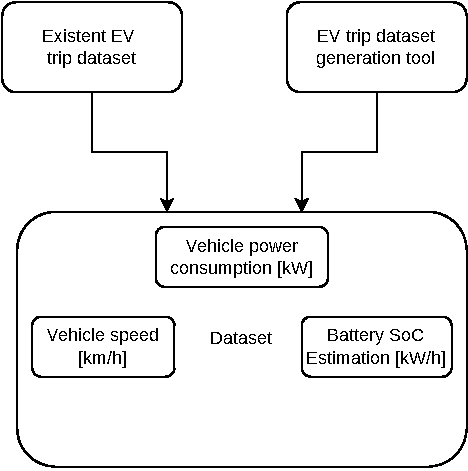
\includegraphics[scale=1.0]{../figures/generic_diagram_dataset_generation_phase}
        \caption{System overview - Dataset generation.}
        \label{fig:generic_diagram_dataset_generation_phase}
    \end{center}
\end{figure}

On the Dataset generation phase
\figref{fig:generic_diagram_dataset_generation_phase}
a \gls{dataset} will be created from historical traffic data
from personally recorded vehicle trips, as well as
external existing \glspl{dataset} such as \textit{VED} 
\citep{vedDataset} or \textit{Emobpy}, an external 
library that provides the generation of \gls{EV} 
trip and consumption \gls{timeSeries} \citep{emobpy}.
The resulting dataset contains multiple
trips with their respective vehicle power consumption [kW]
and the vehicle speed [km/h] in a time series format.

\begin{figure}[H]
    \begin{center}
        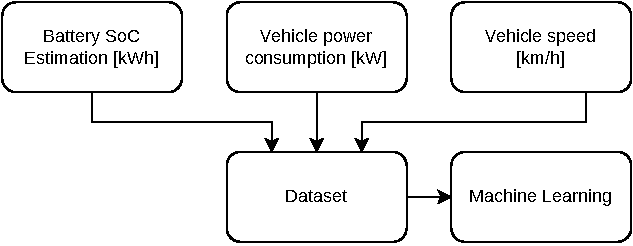
\includegraphics[scale=1.0]{../figures/generic_diagram_learn_phase}
        \caption{System overview - Learning phase.}
        \label{fig:generic_diagram_learn_phase}
    \end{center}
\end{figure}

The generated \gls{dataset} will then be used to train
the model on the Learning phase through machine learning, 
allowing it to learn the estimation of 
the \gls{eRange} for each trip on the \gls{dataset}
as depicted in figure \ref{fig:generic_diagram_learn_phase}.

%! suppress = MissingLabel
% \begin{figure}[H]
%     \begin{center}
%         %! suppress = MissingLabel
%         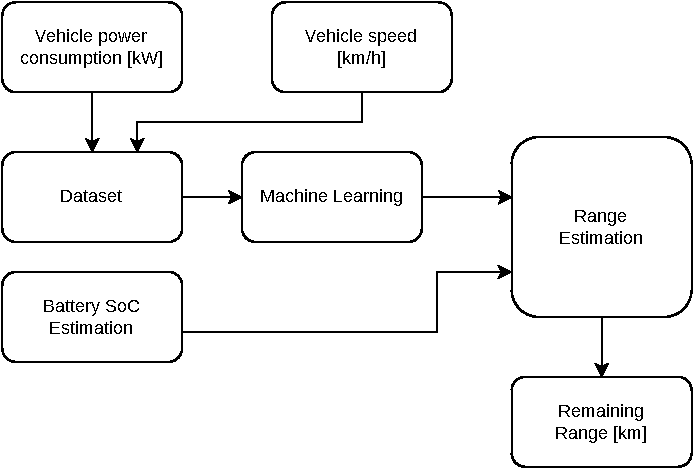
\includegraphics[scale=1.0]{../figures/generic_diagram}
%         \caption{System overview.}
%     \end{center}
% \end{figure}

\begin{figure}[H]
    \begin{center}
        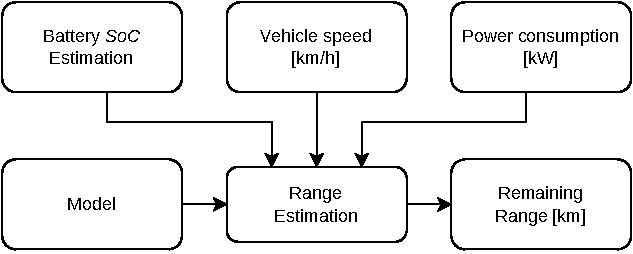
\includegraphics[scale=1.0]{../figures/generic_diagram_estimation_phase}
        \caption{System overview - Estimation phase.}
        \label{fig:generic_diagram_estimation_phase}
    \end{center}
\end{figure}

After training and learning the model with the \gls{dataset},
the Estimation phase performs the \gls{eRange} prediction
on live \gls{SOC} monitoring of a driving \gls{EV}
\figref{fig:generic_diagram_estimation_phase}.

The remainder of this document is structured as follows: 
Chapter \ref{cha:stateOfArt} refers existing solutions 
of the \gls{eRange} estimation problem and their reliance on available
\glspl{dataset} (Section \ref{sec:stateOfArtER}) while
mentioning \gls{machineLearning} and its usability 
in existing \gls{eRange} estimation solutions 
(Section \ref{sec:stateOfArtML}).
On Chapter \ref{cha:planning} will be discussed the 
work state (Section \ref{sec:planningIntro}) followed by 
future work and planning for the next stage 
in the development of this work 
(Section \ref{sec:planningPlanning}). 